\documentclass{beamer}
\usepackage{beamerthemesplit}
\usepackage{wrapfig}
\usetheme{SPbGU}
\usepackage{pdfpages}
\usepackage{amsmath}
\usepackage{cmap}
\usepackage[T2A]{fontenc}
\usepackage[utf8]{inputenc}
\usepackage[english,russian]{babel}
\usepackage{indentfirst}
\usepackage{amsmath}
\usepackage{tikz}
\usepackage{multirow}
\usepackage[noend]{algpseudocode}
\usepackage{algorithm}
\usepackage{algorithmicx}
\usetikzlibrary{shapes,arrows}
\usepackage{fancyvrb}
\newtheorem{rutheorem}{Теорема}
\newtheorem{ruproof}{Доказательство}
\newtheorem{rudefinition}{Определение}
\newtheorem{rulemma}{Лемма}
\beamertemplatenavigationsymbolsempty

\title[]{Разработка механизма использования OpenCL-кода \\
в программах на F\#}
\institute[СПбГУ]{
Санкт-Петербургский государственный университет \\
Кафедра системного программирования }

\author[Кирилл Смиренко]{Кирилл Петрович Смиренко, 371 группа \\
  \and
    {\bfseries Научный руководитель:} к.ф.-м.н., доц. С.В. Григорьев}

\date{25 апреля 2017г.}

\definecolor{orange}{RGB}{179,36,31}

\begin{document}
{
\begin{frame}
  \begin{center}
  {
\includegraphics[width=1.5cm]{pictures/SPbGU_Logo.png}}
  \end{center}
  \titlepage
\end{frame}
}

\begin{frame}[fragile]
  \transwipe[direction=90]
  \frametitle{Введение}
  \begin{itemize}
    \item Графические процессоры (GPU) – средство ускорения вычислений
    \item Средства программирования видеопроцессоров: CUDA, OpenCL
    \item Существуют инструменты запуска высокоуровневого кода на GPU
  \end{itemize}
  \begin{itemize}
    \item Потребность использования низкоуровневого кода в ЯВУ
    \begin{itemize}
      \item переиспользование кода – хорошая практика
      \item переписывать специфические конструкции CUDA и OpenCL на высокоуровневом языке общего назначения нецелесообразно
    \end{itemize}
  \end{itemize}
\end{frame}

\begin{frame}
  \transwipe[direction=90]
  \frametitle{Обзор: существующие решения}
  \begin{itemize}
      \item Средства программирования видеопроцессоров в .NET:
      \begin{itemize}
        \item Alea GPU (CUDA)
        \item Brahma.FSharp (OpenCL)
      \end{itemize}
  \end{itemize}

  \begin{itemize}
    \item Средства запуска CUDA-кода из ЯВУ:
    \begin{itemize}
      \item CUSP
      \item ManagedCuda
    \end{itemize}
  \end{itemize}

  \begin{itemize}
    \item Существующие решения не позволяют типизированно вызывать произвольный низкоуровневый код
  \end{itemize}
\end{frame}

\begin{frame}
  \transwipe[direction=90]
  \frametitle{Обзор: провайдеры типов в F\#}
  \begin{itemize}
    \item Генерируют типы данных и встраивает в окружение времени исполнения
    \item Могут использовать параметры при генерации типов
  \end{itemize}

  \begin{itemize}
    \item Преимущества перед кодогенерацией:
    \begin{itemize}
        \item интеграция с пользовательским контекстом
        \item генерация типов происходит одновременно с компиляцией пользовательского кода
    \end{itemize}
    \item Недостатки:
    \begin{itemize}
        \item трудность тестирования
        \item высокая сложность отладки
    \end{itemize}
  \end{itemize}
\end{frame}

\begin{frame}
  \transwipe[direction=90]
  \frametitle{Постановка задачи}
  \textbf{Цель}: добавление возможности переиспользования OpenCL C-кода в Brahma.FSharp

  \textbf{Задачи}:
  \begin{itemize}
    \item Исследовать возможности провайдеров типов F\#
    \item Реализовать лексический и синтаксический анализатор заголовков OpenCL-функций
    \item Обеспечить возможность типизированного вызова OpenCL-функций в коде на F\#
    \item Провести экспериментальные исследования решения
  \end{itemize}
\end{frame}

\begin{frame}
  \transwipe[direction=90]
  \frametitle{Лексический и синтаксический анализатор}
  \textbf{Инструменты}: FsLex, YaccConstructor (язык YARD)

  \textbf{Материалы}:
  \begin{itemize}
  \item грамматика C99
  \item спецификация OpenCL C 2.0
  \end{itemize}

  \textbf{Особенности реализации}:
  \begin{itemize}
    \item Синтаксический анализатор описан S-атрибутной грамматикой в EBNF
    \item Разбираются только заголовки функций
  \end{itemize}
\end{frame}

\begin{frame}
  \transwipe[direction=90]
  \frametitle{Провайдер типов для OpenCL-функций}
  \begin{itemize}
    \item Генерирует F\#-функцию, типизированную так же, как исходная функция на OpenCL C
    \item Провайдер параметризован путём к подгружаемому файлу
    \item Количество функций в подгружаемом файле не ограничено
    \item Поддерживается отображение указателей в C в ссылки либо массивы в F\#
  \end{itemize}

  \begin{figure}[t]
      \centering
      
\includegraphics[width=11cm]{pictures/tp-call.png}
      \caption{Пример использования провайдера типов}
  \end{figure}

  \begin{itemize}
    \item Ядро Brahma.FSharp доработано для передачи подгружаемых функций драйверу OpenCL
  \end{itemize}
\end{frame}

\begin{frame}[t]
  \transwipe[direction=90]
  \frametitle{Эксперименты}
  \begin{itemize}
    \item Исследование работы реализованного модуля с оптимизированным OpenCL-кодом
    \item Перемножение вещественных матриц с использованием барьеров и локальных групп OpenCL
  \end{itemize}
  \begin{itemize}
    \item Сравнение с наивными реализациями на F\# и OpenCL C
  \end{itemize}
\end{frame}

\begin{frame}[t]
  \transwipe[direction=90]
  \frametitle{Эксперименты}
  \begin{itemize}
    \item NVIDIA GeForce GT 755M, тактовая частота GPU 980 МГц, память 2048 МБ
  \end{itemize}
  \begin{center}
      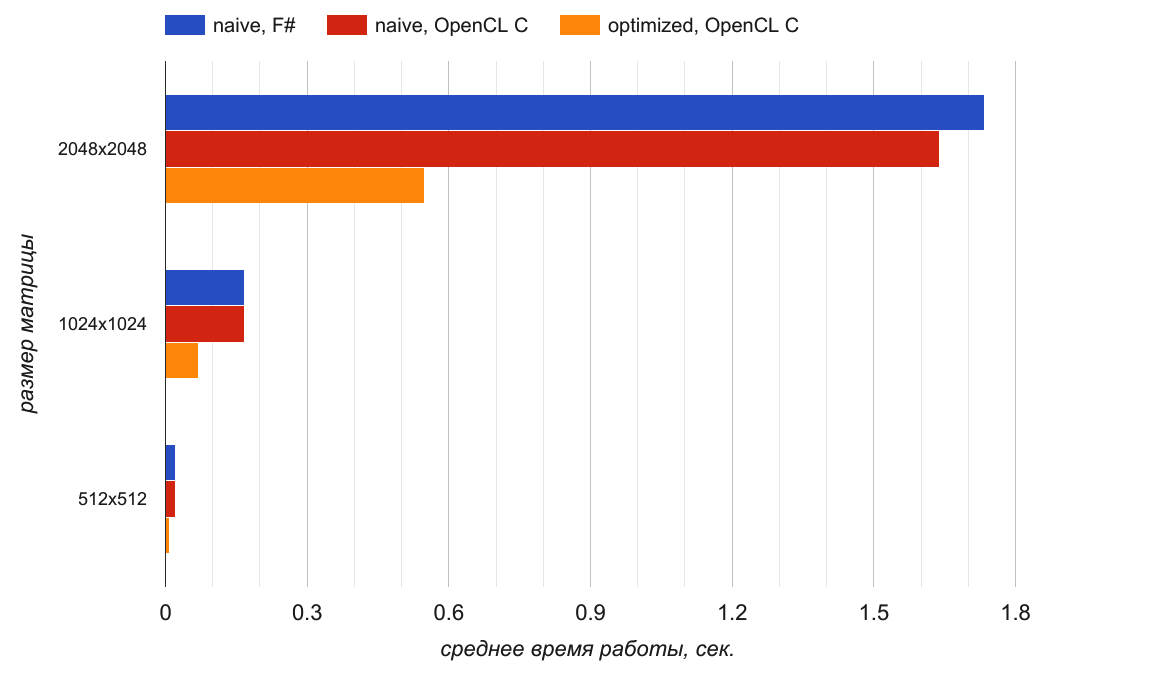
\includegraphics[height=6cm]{pictures/chart.png}
  \end{center}
\end{frame}

\begin{frame}
  \transwipe[direction=90]
  \frametitle{Результаты}
  \begin{itemize}
    \item Исследован механизм провайдеров типов в F\#
    \item Реализован лексический и синтаксический анализатор заголовков OpenCL-функций на языке YARD
    \item Реализован модуль подгрузки исходного кода на OpenCL C в рамках Brahma.FSharp
    \item Проведены экспериментальные исследования работы модуля
  \end{itemize}
\end{frame}

\end{document}
